%-------------------------------------------------------------------------------
%                      Template Naskah Skripsi
%               	Berdasarkan format JTETI FT UGM
% 						(c) @gunturdputra 2014
%-------------------------------------------------------------------------------

%Template pembuatan naskah skripsi.
\documentclass{jtetiskripsi}

\renewcommand \thesection{\Alph{section}.}
\renewcommand \thesubsection{\arabic{subsection}.}

%Untuk prefiks pada daftar gambar dan tabel
\usepackage[titles]{tocloft}
\renewcommand\cftfigpresnum{Gambar\  }
\renewcommand\cfttabpresnum{Tabel\   }

%Untuk hyperlink dan table of content
\usepackage[hidelinks]{hyperref}
\newlength{\mylenf}
\settowidth{\mylenf}{\cftfigpresnum}
\setlength{\cftfignumwidth}{\dimexpr\mylenf+2em}
\setlength{\cfttabnumwidth}{\dimexpr\mylenf+2em}

%Untuk Bold Face pada Keterangan Gambar
\usepackage[labelfont=bf]{caption}

%Untuk caption dan subcaption
\usepackage{caption}
\usepackage{subcaption}

%pdf
\usepackage{pdfpages}

%table
\usepackage{graphics}

\usepackage{wrapfig}

%bibliography
\usepackage{natbib}

%equation
\usepackage{amsmath}

%algoritma
\usepackage{algorithm}
\usepackage{algpseudocode}

%listing
\usepackage{listings}

%-----------------------------------------------------------------
%Disini awal masukan untuk data proposal skripsi
%-----------------------------------------------------------------
\titleind{Rancang Bangun Aplikasi \emph{Search Engine} menggunakan \emph{Crawler}, \emph{PageRank}, dan \emph{TF IDF}}

\fullname{Lazuardy Khatulistiwa}

\idnum{1313618008}

%\approvaldate{12 Februari 2019}
%\approvaldate{12 Februari 2019}

\degree{Sarjana Ilmu Komputer}

\yearsubmit{2022}

\program{Ilmu Komputer}

\dept{Ilmu Komputer}

\firstsupervisor{Muhammad Eka Suryana, M. Kom.}
\firstnip{198512232012121002}

\secondsupervisor{Drs. Mulyono, M.Kom.}
\secondnip{196605171994031003}

%-----------------------------------------------------------------
%Disini akhir masukan untuk data proposal skripsi
%-----------------------------------------------------------------

\tolerance=1
\emergencystretch=\maxdimen
\hyphenpenalty=10000
\hbadness=10000

\begin{document}

\cover
%-----------------------------------------------------------------

%-----------------------------------------------------------------
%Disini akhir masukan untuk muka skripsi
%-----------------------------------------------------------------

\tableofcontents 
\addcontentsline{toc}{chapter}{DAFTAR ISI}
\listoffigures
\addcontentsline{toc}{chapter}{DAFTAR GAMBAR}
%\listoftables
%\addcontentsline{toc}{chapter}{DAFTAR TABEL}

\begin{counterpage}
\end{counterpage}
%Disini awal masukan untuk Bab
%-----------------------------------------------------------------
%!TEX root = ./template-skripsi.tex
%-------------------------------------------------------------------------------
% 								BAB I
% 							LATAR BELAKANG
%-------------------------------------------------------------------------------

\chapter{PENDAHULUAN}

\section{Latar Belakang Masalah}
Indonesia memiliki beberapa sumber perikanan salah satunya adalah budidaya ikan air tawar. Budidaya ikan air tawar memerlukan beberapa modal yaitu lahan, prasarana kolam, Pakan, dan Pengetahuan atau skill dalam berbudidaya ikan. Umumnya budidaya ikan air tawar memelihara banyak jenis ikan atau yang disebut pemeliharaan campuran hal ini disebabkan karena terdapatnya berbagai macam makanan untuk berbagai jenis ikan air tawar, walaupun lebih baik memperhatikan mana jenis ikan yang akan dijadikan peliharaan pokok dan mana yang akan dijadikan peliharaan sampingan \citep{infishta2019web}.

%Budidaya ikan air adalah bentuk dari pembudidayaan yang berfokus pada ikan, baik di kolam maupun di tempat lainnya yang bertujuan untuk menghasilkan bahan pangan, ikan hias, maupun rekreasi \citep{infishta2019web}. Salah satu jenis budidayanya adalah budidaya ikan air tawar. Umumnya budidaya ikan air tawar memelihara banyak jenis ikan atau yang di sebut pemeliharaan campuran hal ini disebabkan karena terdapatnya berbagai macam makanan untuk berbagai jenis ikan air tawar, walaupun lebih baik memperhatikan mana jenis ikan yang akan dijadikan peliharaan pokok dan mana yang akan dijadikan peliharaan sampingan. 

Dalam pembudidayaan ikan air tawar diperlukannya pencatatan beberapa indikator yang berguna untuk menilai kelayakan habitat, memantau perkembangan ikan, dan memantau pemberian pakan sehingga bisa memutuskan treatment apa yang akan dilakukan kedepannya untuk mencapai panen yang baik. Beberapa indikator yang perlu di perhatikan adalah kadar oksigen dalam air, pengukuran kadar ph dalam air, DO (Dissolved Oxygen), Suhu, dan Ammonia. Indikator air tersebut berpengaruh terhadap kelayakan habitat ikan air tawar \citep{pramleonita2018parameter}. Di sisi lain pencatatan terhadap kolam, perlakuan kolam, penaburan ikan dan pemberian pakan juga merupakan faktor yang penting untuk dicatat. Perlunya pencatatan terhadap banyak indikator secara berulang dan intensif menjadi faktor diperlukannya sistem modern yang membantu mempermudah pekerjaan tersebut.

Di Indonesia terdapat beberapa penelitian sistem modern terkait perikanan yang berkontribusi pada budidaya perikanan oleh \citep{supriyati2018sakemkm} melakukan penelitian yang menghasilkan sistem akuntansi budidaya perikanan berbasis android. Penelitian ini dilakukan untuk memecahkan suatu masalah pada pencatatan secara tradisional yang dilakukan oleh petani perikanan yang menyebabkan kurang maksimalnya income yang didapat. Sistem yang dibuat akan digunakan oleh beberapa stakeholders diantaranya adalah: Ketua dari perikanan tersebut, Sekertaris, Bendahara, Seksi sarana produksi, Seksi pengadaan, dan Seksi pemasaran. Sistem ini menerapkan beberapa fitur yaitu Transaksi jual-beli, kas keluar-masuk, dan pembukuan. \citep{Widhiastika2021foklik} melakukan penelitian yang berjudul "Perancangan Aplikasi Jual Beli Produk Perikanan Berbasis Mobile Android". Aplikasi tersebut memungkinkan pengguna dalam melakukan transaksi jual beli perikanan. Aplikasi juga menyediakan wadah untuk diskusi dan informasi gizi dari suatu produk perikanan. Dari dua penelitian sebelumnya didapatkan sistem yang dibuat membantu petani perikanan dalam kegiatan pembukuan transaksi, namun tidak dengan kegiatan aktivitas budidaya.

Penelitian pada sektor IoT pemantauan kualitas air secara real-time dilakukan oleh \citep{Yunior2019MonitoringKualitasAir} yang mana menghasilkan IoT monitoring kualitas air terintegrasi oleh database server. Indikator yang dicatat adalah Ph, Dissolved Oxygen (DO), Suhu, dan Turbidity. IoT dibuat menggunakan microcontroller Arduino, yang mana perannya adalah mengirim data dari sensor dengan protokol GSM ke database server. Pada server juga terdapat halaman yang menampilkan monitoring data berdasarkan database. Penelitian \citep{Rifai2021IoTNodeRed} menghasilkan IoT untuk Pemantauan dan Kontrol otomatis kualitas air berbasis IoT menggunakan Node-Red untuk budidaya udang. Dalam penerapannya indikator yang diukur sama dengan apa yang diukur dalam penelitian \citep{Yunior2019MonitoringKualitasAir} namun dengan tambahan pengukuran ketinggian air. Nantinya setiap sensor terhubung dengan microcontroller arduino, namun pada penelitian \citep{Rifai2021IoTNodeRed} memilih menggunakan NodeMCU (modul wifi) untuk terhubung ke internet. Server yang dibangun menggunakan Node-Red yang merupakan tools yang mempermudah membangun sistem berbasis IoT. Saat pengiriman data ke server arduino menggunakan protokol MQTT yang menerapkan konsep publish dan subscribe. Pada alat kontrol aktuator terdiri dari NodeMCU dan relay dan berguna sebagai pengontrol pompa air dan aerator. Dari dua penelitian diatas terdapat beberapa masalah terkait device IoT terutama pada sensor Ph dan DO. Keakuratan sensor Ph dan DO didasarkan pada grade sensor, semakin tinggi grade sensor semakin mahal sensor tersebut. Sensor Ph dan Do juga mengalami penurunan kualitas seiring waktu berjalan, maka dari itu diperlukannya replacement berkala selambat-lambatnya 1 bulan sekali.

Penelitian IoT pemberian pakan otomatis dilakukan oleh \citep{Setiawan2022IoTSekolahVokasi} yang menghasilkan suatu alat pemberian pakan otomatis. Alat pemberian pakan dapat bekerja secara otomatis berdasarkan waktu yang telah di jadwalkan. IoT yang diterapkan menggunakan NodeMCU sebagai modul yang bisa mengakses jaringan wifi dan blynk sebagai middleware untuk memonitoring pemberian pakan, persediaan pakan,pengaturan jadwal dan takaran pakan. Dalam kasus IoT pemberian pakan otomatis terdapat beberapa kendala yaitu resiko tidak meratanya pemberian pakan karena terbatasnya jangkauan pelemparan pakan. Selanjutnya adalah pelemparan pakan otomatis pada praktiknya ditetapkan oleh jadwal sedangkan dosis pakan bisa berubah tergantung dengan keadaan di lapangan.


% Pengembangan sistem ini dilakukan berdasarkan kebutuhan pengecekan dan pencatatan bebrapa indikator untuk budidaya ikan air tawar yaitu pengecekan kadar ph, DO (Dissolved Oxygen), suhu, pencatatan tebar ikan dan pemberian pakan. Pengembangan sistem yang akan dilakukan yaitu Pengembangan web service berbentuk REST API, yang mana memungkinkan web service tersebut untuk menerima, menyimpan, serta monitoring data melalu user device.

% Web services adalah mekanisme komunikasi dua aplikasi atau mesin yang tidak terikat pada  arsitektur dan teknologi yang dipakai antar dua mesin tersebut \citep{reinert2019web}. Metode web service ada dua macam yaitu SOAP dan REST. SOAP (Simple Object Access Protocol) adalah standar untuk bertukar pesan-pesan berbasis XML melalui jaringan komputer atau sebuah jalan untuk program yang berjalan pada suatu sistem operasi (OS) untuk berkomunikasi dengan program pada OS yang sama maupun berbeda dengan menggunakan HTTP dan XML sebagai mekanisme untuk pertukaran data, maka SOAP dapat berkomunikasi dengan berbagai aplikasi meskipun terdapat perbedaan sistem operasi, teknologi, dan bahasa pemrogramannya \citep{feridi2016web}. REST(REpresentational State Transfer) merupakan standar arsitektur komunikasi berbasis web yang sering diterapkan dalam pengembangan layanan berbasis web. Umumnya menggunakan HTTP(Hypertext Transfer Protocol) sebagai protocol untuk komunikasi data. REST pertama kali diperkenalkan oleh Roy Fielding pada tahun 2000 \citep{feridi2019web}.

Dari beberapa penelitian diatas, penelitian ini bertujuan untuk memberikan solusi dari setiap permasalahan yang ada pada perikanan modern. Fokus penelitian ini adalah membangun arsitektur aplikasi budidaya perikanan modern pada backend yang dapat melayani transaksi query dari berbagai platform. Penelitian ini selanjutnya akan terus dikembangkan dari berbagai sisi antara lain adalah frontend, AI, dll. Berikut beberapa penelitian yang telah dilakukan untuk berkontribusi pada perikanan modern ini.

Penelitian yang terkait dalam penelitian ini adalah penelitian bidang Monitoring data sensing pada budidaya ikan air tawar sudah dilakukan oleh Fadhilah Perwira Hadi dalam penelitian yang berjudul "Rancang Bangun Web Service dan Website sebagai Storage Engine dan Monitoring Data Sensing". Penelitian tersebut menghasilkan suatu sistem web service yang dapat menerima dan memonitoring data yang dikirimkan oleh embedded device, dengan menerapkan konsep IoT \citep{fadhilah2021skripsi}. Pada dasarnya web service yang dirancang oleh \citep{fadhilah2021skripsi} dikhususkan untuk tersambung kepada embedded device IoT. Embedded device sebagai perangkat sensor terhadap beberapa data-data indikator unsur dalam kolam serta mengirim data tersebut ke web service. Penelitian lainnya yang terkait adalah penelitian yang dilakukan oleh \citep{nugraha2022ekstrasiLatarDepan} yang berjudul "Ekstraksi Latar Depan pada Citra Ikan dengan Metode GrabCut yang Diautomasi Menggunakan Saliency Map" yang bertujuan untuk membangun sistem yang memisahkan antara latar depan dan latar belakang pada citra ikan. Penelitian selanjutnya adalah penelitian dengan judul "Fish Movement Tracking dengan Menggunakan Metode GMM dan Kalman Filter" yang dilakukan oleh \citep{alim2022fishmovement} yang bertujuan untuk membangun sebuah sistem yang dapat melakukan pelacakan pergerakan ikan yang diharapkan nantinya dapat dikembangkan kembali untuk sistem penghitungan ikan. Ke 3 penelitian tersebut merupakan kontribusi yang kedepannya akan diterapkan bersamaan dalam penelitian ini kedalam sistem induk.

%yang terkait dengan penelitian ini memiliki kontribusi pada sektor yang sama, yaitu perikanan modern. Dan fokus kontribusi penelitian ini adalah memberikan solusi terhadap beberapa kendala Embedded device IoT serta mengembangakan serta meningkatkan sistem yang sudah ada yang dikembangkan oleh Fadhilah Perwira Hadi, dimana pengembangan berfokus pada web service untuk penerimaan, penyimpanan, dan monitoring data dari user device seperti smartphone, computer, dan tablet.


\section{Rumusan Masalah}
Berdasarkan latar belakang penelitian ini, maka perumusan masalah pada penelitian ini adalah “Bagaimana merancang Arsitektur Aplikasi Budidaya Perikanan Modern pada Backend yang Bertanggung Jawab dalam Melayani Transaksi Query Webservice”.

\section{Pembatasan Masalah}
Adapun beberapa pembatasan masalah yang bertujuan agar penelitian ini lebih terarah dan sesuai dengan tujuan penelitian:
\begin{enumerate}
	\item Sistem yang akan dibangun adalah web service atau biasa disebut backend.
	\item Webservice dikembangkan khusus untuk 1 mitra, dalam hal ini UD JFarm Teknologi. Hanya untuk 1 user.
\end{enumerate}

\section{Tujuan Penelitian}
Penelitian yang dilakukan bertujuan untuk merancang arsitektur aplikasi budidaya perikanan modern pada backend yang bertanggung jawab dalam melayani transaksi query webservice.

\section{Manfaat Penelitian}
\begin{enumerate}
	\item Bagi sektor perikanan
	
	Hasil perancangan arsitektur backend server ini dapat memberikan kontribusi terhadap sistem perikanan modern dalam bentuk web service yang dapat terhubung dengan multi platform.
	
	\item Bagi penulis
		
	Menambah pengetahuan dibidang pengembangan web service khususnya pengembangan Arsitektur BackEnd REST API, mengasah kemampuan \emph{programming}, dan memperoleh gelar sarjana dibidang Ilmu Komputer. Selain itu, penulisan ini juga merupakan media bagi penulis untuk mengaplikasikan ilmu yang didapat di kampus ke kehidupan masyarakat.
		
	\item Bagi Universitas Negeri Jakarta 
	 	
	Menjadi pertimbangan dan evaluasi akademik khususnya Program Studi Ilmu Komputer dalam penyusunan skripsi sehingga dapat meningkatkan kualitas akademik di program studi Ilmu Komputer Universitas Negeri Jakarta serta meningkatkan kualitas lulusannya.
	 			
\end{enumerate} 


% Baris ini digunakan untuk membantu dalam melakukan sitasi
% Karena diapit dengan comment, maka baris ini akan diabaikan
% oleh compiler LaTeX.
\begin{comment}
\bibliography{daftar-pustaka}
\end{comment}

 %!TEX root = ./template-skripsi.tex
%-------------------------------------------------------------------------------
%                            BAB II
%               KAJIAN TEORI
%-------------------------------------------------------------------------------

\chapter{KAJIAN PUSTAKA} 

\section{Perikanan modern}
Perikanan modern adalah pendekatan dalam industri perikanan yang melibatkan penggunaan teknologi canggih, manajemen yang efisien, dan prinsip-prinsip berkelanjutan untuk memaksimalkan produksi ikan dan produk-produk perikanan, sambil tetap menjaga keseimbangan ekosistem dan menjaga sumber daya alam \citep{kusuma2004sistem}.

Perikanan modern melibatkan penerapan teknologi seperti pemantauan satelit, sistem informasi geografis (GIS), penggunaan peralatan nirkabel, penggunaan kapal tangkap yang lebih efisien dan ramah lingkungan, pengelolaan data untuk mengoptimalkan produksi, budidaya ikan secara intensif (aquaculture), serta penerapan praktik-praktik manajemen berkelanjutan yang melibatkan perlindungan terhadap lingkungan laut, pemantauan dan pengelolaan stok ikan, serta penegakan regulasi dan kebijakan.

\section{Sistem backend yang bertanggung jawab untuk melayani transaksi query}

Sistem backend yang bertanggung jawab untuk melayani transaksi query dalam konteks pengembangan perangkat lunak sering disebut sebagai "Query Backend System" atau "Query Processing System." Ini adalah komponen yang mengelola permintaan query dari frontend (pengguna atau aplikasi) dan berinteraksi dengan basis data atau penyimpanan data untuk mengambil, memanipulasi, dan mengembalikan hasil yang relevan \citep{prayogi2021rancang}.

Fungsi utama dari Query Processing System adalah untuk menerima permintaan query (pertanyaan atau perintah) dari pengguna atau aplikasi, menganalisis query tersebut, mengeksekusi operasi yang sesuai pada basis data, dan menghasilkan hasil yang relevan. Proses ini melibatkan beberapa langkah untuk mengoptimalkan kinerja dan efisiensi eksekusi query.


\section{\emph{Scrum}}
\emph{Scrum} merupakan kerangka kerja ringan yang dapat menghasilkan solusi yang adaptif untuk masalah yang kompleks bagi orang, tim, dan organisasi. Kerangka kerja scrum dibiarkan tidak lengkap, hanya mendefinisikan bagian-bagian yang diperlukan untuk mengimplementasi teori \emph{scrum}, selebihnya kecerdasan kolektif orang-orang yang menggunakan \emph{scrum} akan membangun \emph{scrum} itu sendiri. \emph{Scrum} tidak memberikan instruksi yang terperinci kepada setiap anggota tim, melainkan memandu hubungan dan interaksi mereka.

\emph{Scrum} terus berkembang dengan adanya pengalaman dan pemikiran, lalu menghasilkan suatu keputusan berdasarkan pengamatan. Menggunakan proses iterasi dan perlahan menambahkan sesuatu, untuk mengendalikan risiko dan membuat sesuatu dapat diprediksi.

\emph{Scrum} menggunakan prinsip pendekatan \emph{Agile} untuk dapat mengatasi segala macam masalah secara kreatif dan adaptif. Berbagai proses, teknik dan metode dapat digunakan dalam kerangka kerja. 

\emph{Scrum} menggabungkan empat aktivitas formal untuk memeriksa dan mengadaptasi menjadi satu aktivitas konten, \emph{Sprint}. Kegiatan ini dapat berhasil jika menerapkan pilar empiris transparansi, inspeksi, dan adaptasi \emph{Scrum}. 

\begin{enumerate}
	\item Transparansi
	
	Proses dan pekerjaan yang muncul harus dapat dilihat oleh mereka yang melakukan pekerjaan dan mereka yang menerimanya. Untuk \emph{Scrum}, sangat penting bahwa keputusan didasarkan pada kondisi tiga komponen formal, dan komponen \emph{Scrum} dengan transparansi rendah mengurangi nilai dan meningkatkan risiko.
		
	\item Inspeksi
		
	Artefak \emph{scrum} dan kemajuan menuju tujuan yang disepakati harus dirombak secara berkala untuk mendeteksi kemungkinan perbedaan atau masalah yang tidak terduga. Untuk membantu inspeksi, \emph{Scrum} menyediakan ritme dalam bentuk lima acaranya.

	Centang untuk memungkinkan adaptasi. Inspeksi tanpa adaptasi dianggap tidak berguna. Aktivitas \emph{scrum} dirancang untuk menginspirasi perubahan.	
		
	\item Adaptasi
	
	Jika ada aspek proses yang menyimpang dari batas yang dapat diterima, atau jika produk yang dihasilkan tidak dapat diterima, proses yang diterapkan atau bahan yang dihasilkan harus disesuaikan. Penyesuaian harus dilakukan sesegera mungkin untuk meminimalkan penyimpangan lebih lanjut.

	Adaptasi menjadi lebih sulit ketika orang-orang yang terlibat tidak diberdayakan atau dikelola sendiri. Tim \emph{scrum} diharapkan untuk menyesuaikan diri saat mereka mempelajari hal-hal baru melalui inspeksi.

\end{enumerate}

	\subsection{Tim Scrum}
	
	Unit dasar \emph{Scrum} adalah tim kecil. \emph{Scrum Team} terdiri dari \emph{Scrum Master}, \emph{Product Owner}, dan \emph{Developer}. Dalam tim \emph{Scrum}, tidak ada sub-tim atau hierarki. Tim \emph{scrum} bersifat lintas fungsi, yang berarti bahwa anggota memiliki semua keterampilan yang mereka butuhkan untuk menciptakan nilai di setiap \emph{Sprint}. Tim scrum cukup kecil untuk tetap lincah dan cukup besar untuk menyelesaikan pekerjaan penting dalam sprint, biasanya 10 orang atau kurang.

	Tim \emph{Scrum} bertanggung jawab atas semua aktivitas terkait produk, termasuk kolaborasi pemangku kepentingan, validasi, pemeliharaan, operasi, eksperimen, penelitian dan pengembangan, dan aktivitas lain apa pun yang mungkin diperlukan.

	Seluruh Tim \emph{Scrum} bertanggung jawab untuk menciptakan peningkatan yang berharga dan berguna di setiap \emph{Sprint}. \emph{Scrum} mendefinisikan tiga tanggung jawab khusus dalam Tim \emph{Scrum}: Pengembang, Pemilik Produk, dan \emph{Scrum Master}.
	
	\begin{enumerate}
	
		\item Pengembang (\emph{Developers})
		
		Pengembang adalah seseorang di tim \emph{Scrum} yang bekerja untuk membuat aspek apa pun dari \emph{Increment} yang dapat digunakan oleh setiap Sprint.

		Keterampilan khusus yang dibutuhkan oleh pengembang seringkali luas dan bervariasi menurut bidang pekerjaan. Namun, pengembang selalu bertanggung jawab untuk:
		
		\begin{enumerate} [a.]
		
			\item Mengembangkan rencana untuk \emph{Sprint}, \emph{Sprint Backlog};

			\item Menanamkan kualitas dengan tetap berpegang pada definisi selesai;

			\item Menyesuaikan rencana harian mereka untuk mencapai \emph{Sprint Goals}; dan,

			\item Sebagai profesional, kami memikul tanggung jawab satu sama lain.
		
		\end{enumerate}
		
		\item Pemilik Produk (\emph{Product Owner})
		
		Pemilik Produk bertanggung jawab untuk memaksimalkan nilai produk yang dikembangkan oleh Tim \emph{Scrum}. Bagaimana hal ini dicapai akan bervariasi antara perusahaan, tim, dan individu. \emph{Product Owner} juga bertanggung jawab untuk mengelola \emph{Product Backlog} dengan baik, termasuk:
		
		\begin{enumerate} [a.]
		
			\item Mengembangkan dan mengkomunikasikan tujuan produk dengan jelas;

			\item Membuat dan mengkomunikasikan item backlog produk dengan jelas; 
			
			\item Memesan backlog produk; dan,

			\item Pastikan \emph{Product Backlog} transparan, terlihat, dan mudah dipahami.
		
		\end{enumerate}
		
		Pemilik Produk dapat melakukan pekerjaan yang dijelaskan di atas atau mendelegasikan tanggung jawab kepada orang lain. Seluruh organisasi harus menghormati keputusan mereka. Keputusan ini tercermin dalam konten dan urutan \emph{Product Backlog}, dan melalui peningkatan yang dapat diperiksa di \emph{Sprint Review}.

		Pemilik Produk adalah orang, bukan panitia. Pemilik Produk dapat mewakili kebutuhan banyak pemangku kepentingan dalam \emph{Product Backlog}. Siapapun anggota tim yang ingin mengubah \emph{Product Backlog} dapat melakukannya dengan mencoba meyakinkan Pemilik Produk.
		
		\item \emph{Scrum Master}
		
		\emph{Scrum Master} bertanggung jawab untuk membangun \emph{Scrum} sebagaimana didefinisikan dalam Panduan \emph{Scrum}. Mereka melakukan ini dengan membantu semua orang di tim dan organisasi \emph{Scrum} memahami teori dan praktik \emph{Scrum}.

		\emph{Scrum Master} bertanggung jawab atas efektivitas Tim \emph{Scrum}. Mereka melakukan ini dengan meminta tim \emph{Scrum} meningkatkan praktik mereka dalam kerangka kerja \emph{Scrum}.

		\emph{Scrum Masters} adalah pemimpin sejati yang melayani Tim \emph{Scrum} dan organisasi yang lebih besar.

		\emph{Scrum Master} melayani Tim Scrum dengan cara, seperti:
		
		\begin{enumerate}[a.]
		
			\item Melatih anggota tim dalam manajemen diri dan manajemen berbagai bidang;

			\item Bantu tim \emph{Scrum} fokus pada penciptaan peningkatan bernilai tinggi yang memenuhi definisi selesai;

			\item Buka blokir kemajuan Tim \emph{Scrum}; dan,

			\item Pastikan semua acara \emph{Scrum} terjadi, positif, produktif, dan sesuai jadwal.
		
		\end{enumerate}
		
		\emph{Scrum Master} melayani Pemilik Produk dengan cara, seperti:
		
		\begin{enumerate}[a.]
		
			\item Membantu menemukan teknik untuk definisi tujuan produk yang efektif dan manajemen simpanan produk;

			\item Membantu tim \emph{Scrum} memahami kebutuhan akan item \emph{Product Backlog} yang jelas dan ringkas;

			\item Membantu membangun program produk empiris untuk lingkungan yang kompleks; dan,

			\item Memfasilitasi kolaborasi pemangku kepentingan sesuai kebutuhan atau kebutuhan.
		
		\end{enumerate}
		
		\emph{Scrum Master} melayani organisasi dengan cara, seperti:
		
		\begin{enumerate}[a.]
		
			\item Memimpin, melatih dan melatih organisasi dalam implementasi \emph{Scrum};

			\item Merencanakan dan merekomendasikan penerapan \emph{Scrum} dalam organisasi;

			\item Membantu karyawan dan pemangku kepentingan memahami dan menerapkan metode empiris untuk pekerjaan yang kompleks; dan,

			\item Menghilangkan hambatan antara \emph{stakeholder} dan tim \emph{Scrum}.
		
		\end{enumerate}


	\end{enumerate}

	\subsection{Aktivitas-aktivitas Scrum (Scrum Events)}
	
	\emph{Sprint} adalah wadah untuk semua acara lainnya. Setiap acara di \emph{Scrum} adalah kesempatan formal untuk meninjau dan menyesuaikan artefak \emph{Scrum}. Acara-acara ini secara khusus dirancang untuk mencapai transparansi yang diperlukan. Kegagalan untuk mengoperasikan acara apapun seperti yang ditentukan menghasilkan kesempatan yang hilang untuk peninjauan dan adaptasi. Acara digunakan di \emph{Scrum} untuk menciptakan ketertiban dan meminimalkan kebutuhan akan rapat yang tidak ditentukan dalam \emph{Scrum}. Idealnya, semua acara diadakan pada waktu dan tempat yang sama untuk mengurangi kerumitan.
	
	\begin{enumerate}
	
		\item \emph{Sprint}
		
		\emph{Sprint} adalah jantung dari \emph{Scrum}, di mana ide-ide diubah menjadi nilai. Mereka adalah acara berdurasi tetap satu bulan atau kurang untuk menciptakan konsistensi. \emph{Sprint} baru dimulai segera setelah \emph{Sprint} sebelumnya berakhir.

		Semua pekerjaan yang diperlukan untuk mencapai Tujuan Produk, termasuk Perencanaan \emph{Sprint}, \emph{Scrum} Harian, Ulasan \emph{Sprint}, dan Retrospektif \emph{Sprint}, terjadi selama:
		
		\begin{enumerate}[a.]
		
			\item tidak membuat perubahan apa pun yang akan membahayakan \emph{Sprint Goal};

			\item Kualitas tidak berkurang;

			\item \emph{Product Backlog} sedetail yang dibutuhkan; dan,

			\item Semakin banyak yang dipelajari, ruang lingkup dapat diklarifikasi dan dinegosiasikan ulang dengan Pemilik Produk.
		
		\end{enumerate}
		
		\emph{Sprint} memungkinkan prediktabilitas dengan memastikan bahwa kemajuan terhadap sasaran produk diperiksa dan diakomodasi setidaknya setiap bulan kalender. Ketika Cakrawala Sprint terlalu panjang, Tujuan Sprint mungkin gagal, kompleksitas dapat meningkat, dan risiko dapat meningkat. \emph{Sprint} yang lebih pendek dapat digunakan untuk menghasilkan lebih banyak siklus pembelajaran dan membatasi risiko biaya dan upaya untuk kerangka waktu yang lebih pendek. Setiap \emph{Sprint} dapat dianggap sebagai proyek pendek.

	Berbagai praktik ada untuk memprediksi kemajuan, seperti kelelahan, kelelahan, atau aliran kumulatif. Meskipun terbukti bermanfaat, ini tidak menggantikan pentingnya empirisme. Dalam lingkungan yang kompleks, apa yang terjadi tidak diketahui. Hanya apa yang telah terjadi yang dapat digunakan untuk keputusan berwawasan ke depan. \emph{Sprint} dapat dibatalkan jika \emph{Sprint Goals} sudah kedaluwarsa. Hanya Pemilik Produk yang berhak membatalkan Sprint.
		
		\item Perencanaan \emph{Sprint}
		
		Perencanaan \emph{Sprint} memulai \emph{Sprint} dengan meletakkan pekerjaan yang harus dilakukan untuk \emph{Sprint}. Rencana akhir dibuat secara kolaboratif oleh seluruh tim \emph{Scrum}.

		\emph{Product Owner} memastikan bahwa peserta siap untuk mendiskusikan item \emph{Product Backlog} yang paling penting dan bagaimana mereka memetakan ke tujuan produk. Tim \emph{Scrum} juga dapat mengundang orang lain untuk berpartisipasi dalam Perencanaan \emph{Sprint} untuk memberikan saran.
		
		\item \emph{Scrum} harian (\emph{Daily Scrum})
		
		Tujuan dari \emph{Daily Scrum} adalah untuk memeriksa kemajuan terhadap \emph{Sprint Goals} dan menyesuaikan \emph{Sprint Backlog} sesuai kebutuhan untuk menyesuaikan rencana kerja di masa mendatang.

		\emph{Daily Scrum} adalah aktivitas 15 menit untuk pengembang di tim \emph{Scrum}. Untuk mengurangi kompleksitas, ini dilakukan pada waktu dan tempat yang sama setiap hari kerja \emph{Sprint}. Jika \emph{Product Owner} atau \emph{Scrum Master} aktif mengerjakan item di \emph{Sprint Backlog}, mereka berpartisipasi sebagai \emph{developer}.

		Pengembang dapat memilih struktur dan teknik apa pun yang mereka inginkan, selama \emph{Scrum} harian mereka berfokus pada kemajuan Tujuan \emph{Sprint} dan memiliki rencana yang dapat diterapkan untuk hari kerja berikutnya. Ini menciptakan fokus dan meningkatkan manajemen diri.

		\emph{Daily Scrum} dapat meningkatkan komunikasi, mengidentifikasi hambatan, dan memfasilitasi pengambilan keputusan yang cepat, menghilangkan kebutuhan untuk rapat ulang.
		
		\emph{Daily Scrum} bukan satu-satunya waktu pengembang menyesuaikan rencana mereka. Tim sering bertemu sepanjang hari untuk berdiskusi lebih rinci tentang cara menyesuaikan atau merencanakan ulang sisa \emph{print}.
		
		\item Pembahasan \emph{Sprint} (\emph{Sprint Review})
		
		Tujuan dari \emph{Sprint Review} adalah untuk memeriksa hasil \emph{Sprint} dan mengidentifikasi penyesuaian di masa depan. Tim scrum mempresentasikan hasil kerja mereka kepada pemangku kepentingan utama dan mendiskusikan kemajuan menuju tujuan produk.

		Selama acara, Tim \emph{Scrum} dan pemangku kepentingan meninjau apa yang telah dicapai dalam \emph{Sprint} dan bagaimana lingkungan mereka telah berubah. Berdasarkan informasi ini, peserta berkolaborasi tentang apa yang harus dilakukan selanjutnya. \emph{Product Backlog} juga dapat disesuaikan untuk memenuhi peluang baru. Tinjauan \emph{Sprint} adalah rapat kerja dan Tim Scrum harus menghindari membatasinya pada presentasi.

		\emph{Sprint Review} adalah kegiatan \emph{Sprint} kedua dari belakang, dan \emph{Sprint} sebulan tidak melebihi maksimal empat jam. Acara biasanya lebih pendek untuk \emph{Sprint} yang lebih pendek.
				
		\item \emph{Sprint Retrospektif}
		
		Tujuan dari \emph{Sprint Retrospective} adalah untuk merencanakan cara-cara untuk meningkatkan kualitas dan efektivitas.

		Tim \emph{Scrum} memeriksa bagaimana \emph{Sprint} terakhir berjalan sehubungan dengan individu, interaksi, proses, alat, dan Definisi Selesai. Elemen yang diperiksa seringkali berbeda dengan domain pekerjaan. Asumsi yang menyesatkan mereka diidentifikasi dan asal-usulnya dieksplorasi. Tim \emph{Scrum} mendiskusikan apa yang berjalan dengan baik selama \emph{Sprint}, masalah apa yang dihadapi, dan bagaimana masalah tersebut (atau tidak) diselesaikan.

		Tim \emph{Scrum} mengidentifikasi perubahan yang paling membantu untuk meningkatkan efektivitasnya. Perbaikan yang paling berdampak ditangani sesegera mungkin. Mereka bahkan dapat ditambahkan ke \emph{Sprint Backlog} untuk \emph{Sprint} berikutnya.

		\emph{Sprint Retrospective} mengakhiri \emph{Sprint}. Ini dibatasi waktu hingga maksimum tiga jam untuk \emph{Sprint} satu bulan. Untuk \emph{Sprint} yang lebih pendek, acaranya biasanya lebih pendek.
	
	\end{enumerate}

	\subsection{Komponen \emph{Scrum} (\emph{Scrum Artifacts})}
	
	Artefak \emph{scrum} mewakili pekerjaan atau nilai. Mereka dirancang untuk memaksimalkan transparansi informasi penting. Jadi setiap orang yang mengkajinya memiliki dasar yang sama untuk adaptasi.

	Setiap artefak berisi komitmen untuk memastikan bahwa artefak tersebut memberikan informasi yang meningkatkan transparansi dan fokus serta kemajuan yang dapat diukur:
	
	\begin{enumerate}[a.]

		\item Untuk \emph{Product Backlog}, itu adalah tujuan produk.

		\item Untuk \emph{Sprint Backlog}, itu adalah \emph{Sprint Goal}.

		\item Untuk \emph{Increment}, itu adalah definisi penyelesaian.
		
	\end{enumerate}

	Komitmen ini dirancang untuk memperkuat empirisme dan nilai-nilai \emph{Scrum} bagi tim \emph{Scrum} dan pemangku kepentingannya.
	
	\begin{enumerate}[a.]
	
		\item \emph{Product Backlog}
		
		\emph{Product Backlog} adalah daftar berurutan yang muncul dari apa yang dibutuhkan untuk meningkatkan suatu produk. Ini adalah satu-satunya sumber pekerjaan yang dilakukan oleh tim \emph{Scrum}.

		Item \emph{Product Backlog} yang dapat dikerjakan oleh \emph{Scrum Team} dalam sebuah \emph{Sprint} dianggap siap untuk diseleksi dalam aktivitas Sprint Planning. Mereka biasanya mendapatkan transparansi ini setelah kegiatan pemurnian. Penyempurnaan \emph{Product Backlog} adalah tindakan memecah dan mendefinisikan lebih lanjut item \emph{Product Backlog} menjadi item yang lebih kecil dan lebih tepat. Menambahkan detail seperti deskripsi, urutan, dan dimensi adalah aktivitas yang berkelanjutan. Atribut sering bervariasi menurut bidang pekerjaan.

		Pengembang yang akan melakukan pekerjaan bertanggung jawab atas ukurannya. Pemilik produk dapat mempengaruhi pengembang dengan membantu mereka memahami dan memilih pertukaran.
		
		\item \emph{Sprint Backlog}
		
		\emph{Sprint Backlog} mencakup \emph{Sprint Goal} (Mengapa), satu set Item \emph{Product Backlog} yang dipilih untuk \emph{Sprint} (Apa), dan rencana yang layak untuk memberikan \emph{Increment} (Bagaimana).

		\emph{Sprint Backlog} adalah rencana yang dibuat oleh pengembang. Ini adalah gambaran \emph{real-time} yang sangat visual tentang apa yang akan dicapai pengembang selama \emph{Sprint} untuk mencapai Tujuan \emph{Sprint}. Oleh karena itu, \emph{Sprint Backlog} diperbarui sepanjang \emph{Sprint} karena lebih banyak yang dipelajari. Itu harus memiliki detail yang cukup sehingga mereka dapat memeriksa kemajuan mereka di \emph{Scrum} harian.
		
		\item \emph{Increment} (Peningkatan)
		
		\emph{Increment} adalah batu loncatan konkret untuk mencapai tujuan produk. Setiap kenaikan melengkapi semua kenaikan sebelumnya dan divalidasi secara menyeluruh untuk memastikan bahwa semua kenaikan bekerja sama. Untuk memberikan nilai, peningkatan harus tersedia.

		Mungkin ada beberapa peningkatan dalam \emph{Sprint}. Jumlah kenaikan yang disediakan dalam \emph{Sprint Review} mendukung empirisme. Namun, delta dapat dikirimkan ke pemangku kepentingan sebelum akhir \emph{sprint}. Ulasan \emph{sprint} tidak boleh dilihat sebagai cara untuk membuka nilai.

		Pekerjaan tidak dapat dianggap sebagai bagian dari kenaikan kecuali jika memenuhi definisi selesai.	
	\end{enumerate}

\section{REST}

REST adalah arsitektur yang digunakan untuk pemrograman web, dan beroperasi menggunakan protokol HTTP. Arsitektur REST berfokus pada sumber daya, yang masing-masing merupakan komponen terpisah. Sumber daya diakses melalui tautan menggunakan metode HTTP standar, dan setiap klien dan server dalam sistem REST bekerja secara berbeda, klien mengakses dan berinteraksi dengan sumber daya, dan server hanya menyediakan akses ke sumber daya. 

Arsitektur REST adalah arsitektur pengembangan API yang menggunakan hyperlink, header, dan kode status untuk berkomunikasi. Layanan web RESTful adalah layanan web yang dikembangkan menggunakan arsitektur REST. Setiap sumber daya di REST diberi URI atau ID universal. Layanan web RESTful menggunakan metode HTTP untuk menyediakan representasi sumber daya, seperti yang didefinisikan oleh Uniform Resource Identifier. Layanan web menggunakan metode HTTP untuk mengimplementasikan arsitektur REST.

	
	\subsection {URL Design}
	
	Akses RESTful API menggunakan protokol HTTP. Penamaan dan struktur URL yang konsisten akan menghasilkan API yang baik yang mudah dipahami oleh pengembang. URL API sering disebut sebagai titik akhir dalam pemanggilannya.
	
	\subsection {HTTP Verbs}
	
	Setiap permintaan yang dibuat di sana menggunakan metode sehingga server tahu apa yang diminta klien:
	
	\begin{enumerate}[a.]
		
		\item GET
		
		GET adalah metode permintaan HTTP paling sederhana yang digunakan untuk membaca atau mendapatkan data dari suatu sumber.
		
		\item POST
		
		POST adalah metode permintaan HTTP yang digunakan untuk membuat data baru dengan memasukkan data ke dalam badan saat membuat permintaan.
		
		\item PUT
		
		PUT adalah metode permintaan HTTP yang biasanya digunakan untuk memperbarui data sumber daya.
		
		\item DELETE
		
		DELETE adalah metode permintaan HTTP yang digunakan untuk menghapus data dari sumber daya.

	\end{enumerate}
	
	\subsection {HTTP Response Code}
	
	Kode respons HTTP adalah kode standar yang memberitahu klien tentang hasil permintaan. Secara umum, ada 3 kode grup yang sering dijumpai di RESTful API, yaitu:
	
	\begin{enumerate}[a.]
	
		\item 2XX : adalah kode respon yang menunjukkan bahwa permintaan berhasil.
		\item 4XX : adalah kode respon yang menunjukkan bahwa permintaan mengalami kesalahan di sisi klien.
		\item 5XX: adalah kode respon, yang menunjukkan bahwa permintaan mengalami kesalahan di sisi server.
	
	\end{enumerate}
	
    	\subsection {Format Response}
	
	Setiap permintaan yang dibuat, klien akan menerima data respons dari server, biasanya dalam bentuk data XML atau JSON. Setelah klien memiliki data respons, klien dapat menggunakannya dengan menguraikan data dan memprosesnya sesuai kebutuhan.
	
\section{MongoDB}

	MongoDB adalah sistem manajemen basis data yang dirancang untuk internet dan aplikasi berbasis web. MongoDB adalah database NoSQL berbasis dokumen. Model data dokumen MongoDB membuatnya mudah untuk dibuat aktif, karena memiliki dukungan untuk data tidak terstruktur. Dokumen MongoDB dikodekan dalam format seperti JSON, yang disebut BSON. BSON sangat cocok untuk objek modern metodologi pemrograman berorientasi dan ringan dan cepat \citep{hemakrishnan2016mongodb}.
	
	Perbedaan utama antara NoSQL dan \textit{Relational Database Management System} (RDBMS) adalah bagaimana data dimodelkan pada basis data. Pemodelan pada RDBMS masih menggunakan tabel-tabel terstruktur, dimana kolom-kolom pada setiap barisnya tetap satu sama lain, sedangkan pemodelan data pada NoSQL khususnya pada MongoDB menggunakan dokumen-dokumen dimana setiap baris memiliki Kolom-kolom yang berbeda dengan baris lainnya. Contoh perbedaan konseptual database antara RDBMS dan NoSQL ditunjukkan pada \textbf{Gambar \ref{fig:pemodelan_rdbms}} (Pemodelan RDBMS) dan \textbf{Gambar \ref{fig:pemodelan_nosql}} (Pemodelan NoSQL).
\begin{figure}[H]
	\centering
	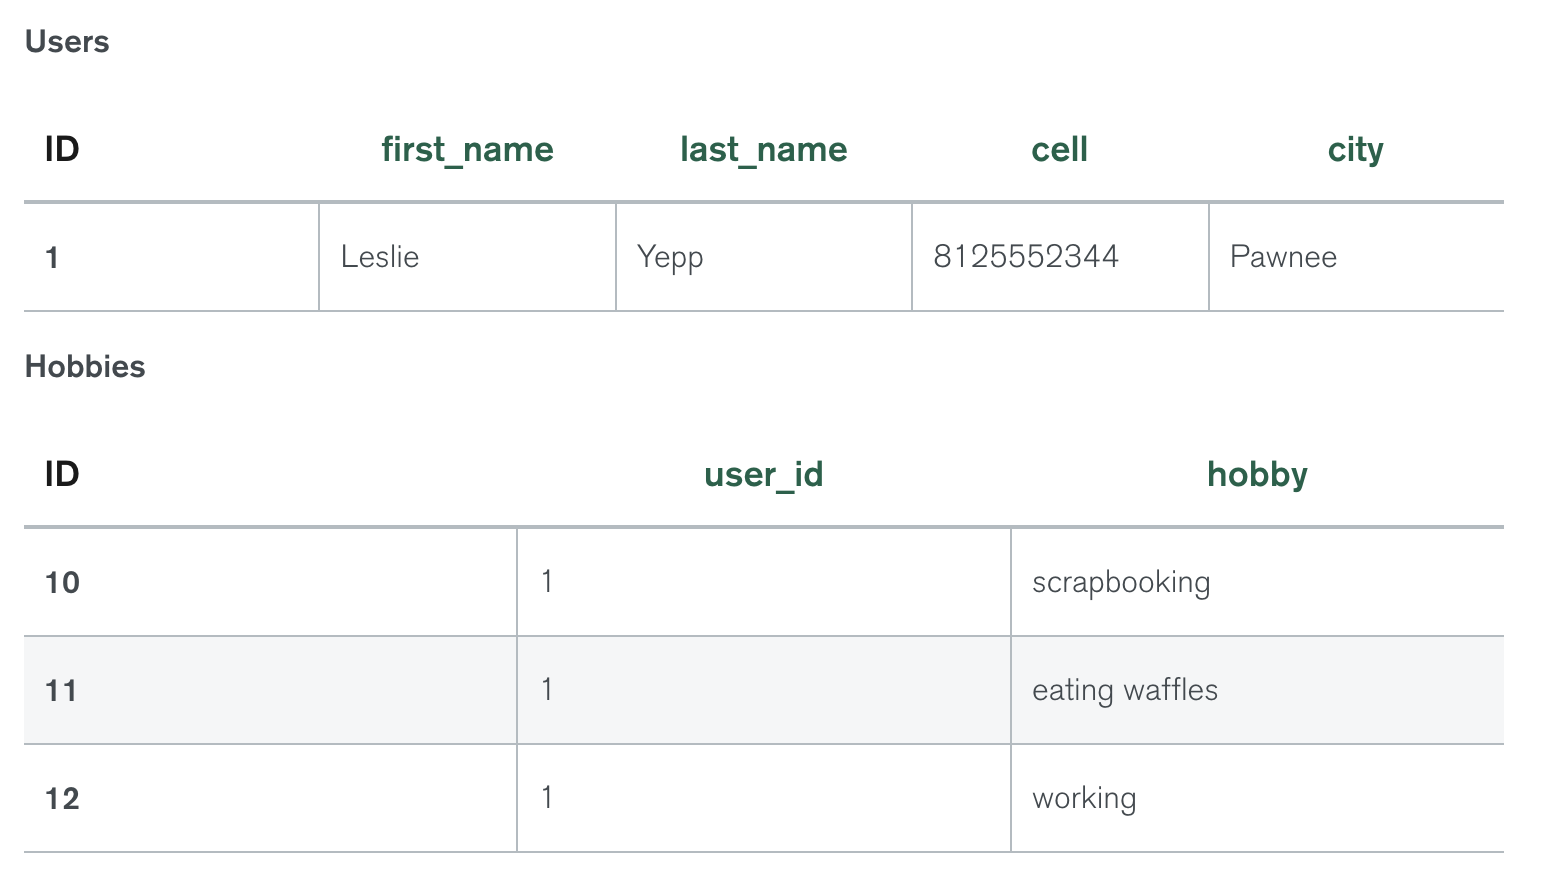
\includegraphics[width=1\textwidth]{gambar/pemodelan_rdbms.png}
	\captionsource{Pemodelan RDBMS}{\href{https://www.mongodb.com/nosql-explained}{\textit{https://www.mongodb.com/nosql-explained}}}
	\label{fig:pemodelan_rdbms}
\end{figure}
\begin{figure}[H]
	\centering
	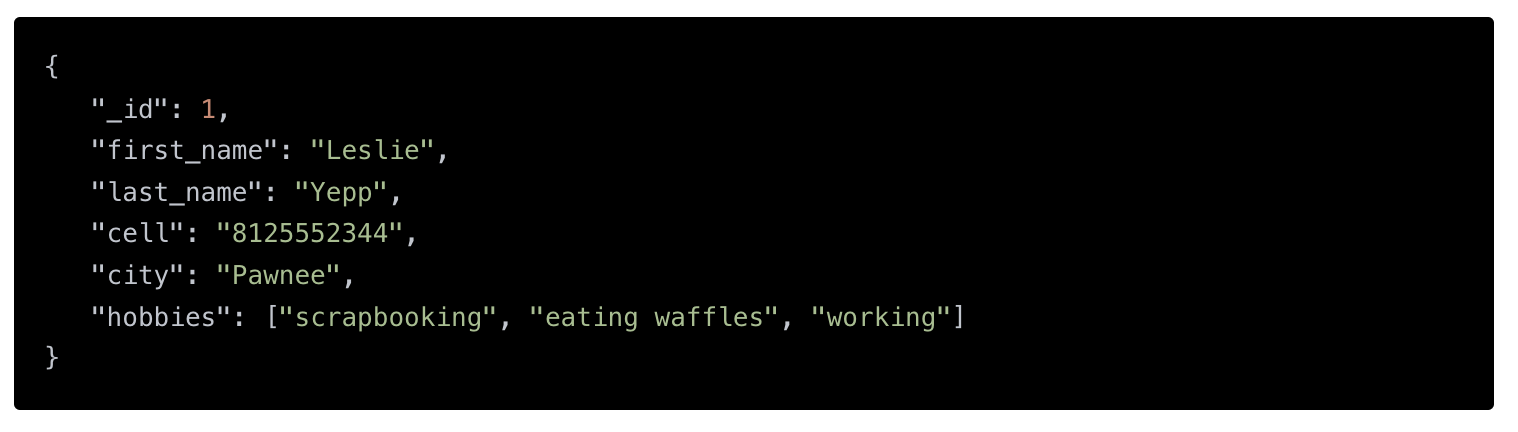
\includegraphics[width=1\textwidth]{gambar/pemodelan_nosql.png}
	\captionsource{Pemodelan NoSQL}{\href{https://www.mongodb.com/nosql-explained}{\textit{https://www.mongodb.com/nosql-explained}}}
	\label{fig:pemodelan_nosql}
\end{figure}
	
	Menurut Gambar \ref{fig:pemodelan_rdbms}, untuk menyimpan data \textit{user} dan data \textit{hobby}, diperlukan dua tabel terpisah, sedangkan dalam pemodelan NoSQL Gambar \ref{fig:pemodelan_nosql}, data \textit{user} dan \textit{hobby} dalam satu dokumen yang sama. Dengan NoSQL, ketika ingin mengambil dua bagian data secara bersamaan, hanya memerlukan satu dokumen tanpa gabungan, yang menghasilkan kueri lebih cepat daripada RDBMS.
	
	Meskipun NoSQL, desain database masih harus dilakukan. Desain basis data memungkinkan untuk mengonfirmasi dan mendokumentasikan pemahaman tentang basis data dan memastikan bahwa orang-orang melihat lanskap informasi dengan cara yang sama. Dengan kata lain, desain database adalah alat komunikasi. Berikut merupakan komparasi dari RDBMS dan NoSQL \textbf{Table \ref{table:komparasi_database}} \citep{Kunda2017ACS}.
	
	
\begin{table}[H]
	\centering
	\caption{\textit{Komparasi Database RDBMS dan NoSQL}}
	\label{table:komparasi_database}
	\begin{tabular}{@{} |p{0.5cm}|p{2cm}|p{5cm}|p{5cm}| @{}}
		\hline
		\textbf{No} & \textbf{Kriteria} & \textbf{RDBMS} & \textbf{NoSQL} \\
		\hline
		1 & Variety &  Terdapat dalam jenis open source dan close platform & Kebanyakan dalam bentuk open source\\
		\hline
		2 & Scalability &  Meningkatkan performa dengan meningkatkan hardware dalam server & Meningkatkan dengan cara horizontal atau menambah server\\
		\hline
		3 & Cost &  Lebih mahal mengingat harusnya penambahan hardware & Lebih murah mengingat murahnya upgrade secara horizontal \\
		\hline
		4 & Volume of Data &  Menangani data yang terbatas & Menangani data yang lebih besar\\
		\hline
		5 & Performance &  Lebih lambat karena perlunya memproses informasi  & Memiliki query performance lebih baik\\
		\hline
		6 & Complexity &  Lebih kompleks karena memerlukan normalisasi hubungan antara tabel & lebih flexible dapat menyimpan struktur yang berbeda dalam satu collections\\
		\hline
		7 & Consistency &  Dengan skema yang kompleks menjadikannya lebih konsisten & Kurang konsisten dikarenakan skema yang bermacam-macam\\
		\hline
		8 & Security &  Memiliki mekanisme keamanan yang baik untuk melindungi data & Keamanan ditangani oleh middleware dan bukan bagian dari database\\
		\hline
	\end{tabular}
\end{table}

\section{Flask Framework}

Framework adalah kerangka kerja untuk mengembangkan aplikasi berbasis web dan desktop. Kerangka kerja di sini sangat membantu pengembang untuk menulis hal-hal yang lebih terstruktur dan rapi.

Framework ini dibuat untuk menyederhanakan kinerja bagi pemrogram. Jadi programmer tidak perlu menulis kode berulang-ulang. Karena hanya perlu mengkompilasi komponen pemrograman itu sendiri \citep{robithadani2020framework}.

Flask Framework merupakan kerangka kerja yang berbasis web. Flask dibangun diatas bahasa pemrograman python dengan menggunakan dependensi Werkzeug dan Jinja2. Kerangka kerja Flask bersifat mikro karena tidak membutuhkan alat-alat tertentu atau pustaka. Flask mendukung ekstensi yang dapat menambahkan fitur aplikasi seolah-olah mereka diimplementasikan dalam Flask itu sendiri.
	
	
	\subsection {Flask routing}
	
	Routing adalah modul dalam aplikasi yang mengatur pengoperasian aplikasi berbasis web. Route dapat menangani semua perintah yang telah  dideklarasikan. Routing bisa dianalogikan sebagai route diagram penjelas tentang cara menavigasi aplikasi yang sedang dibangun.
	
	App Routing berarti memetakan URL ke fungsi tertentu yang akan menangani logika untuk URL tersebut. Berikut adalah contoh routing di framework flask:

\begin{lstlisting}
from flask import Flask
  
app = Flask(__name__)
  
# Pass the required route to the decorator.
@app.route("/hello")
def hello():
   	return "Hello, Welcome to GeeksForGeeks"
    
@app.route("/")
def index():
    	return "Homepage of GeeksForGeeks"
  
if __name__ == "__main__":
	app.run(debug=True)
\end{lstlisting}

Seperti potongan code di atas pemetaan URL ke fungsi menggunakan decorator sebelum fungsi ditulis. Dan contoh diatas merupakan contoh yang sederhana pada routing. Berikut adalah beberapa hal yang bisa dilakukan flask routing:

\begin{enumerate}[a.]
	\item Route Methods
		
		Pada dasarnya saat melakukan routing, secara default metode yang dipakai adalah GET. Untuk membuat agar URL dapat menggunakan metode lain seperti POST diharuskan mendefinisikan metodenya pada argumen route.
\begin{lstlisting}
@app.route('/home', methods=['POST', 'GET']) 
def home(): 
    return '<h1>Anda berada di halaman beranda!</h1>'
\end{lstlisting}
	\item Route Variables
		
		Meneruskan variables merupakan sebuah fitur dasar yang memungkinkan pengguna mengirimkan informasi melalui URL. Untuk mengimplementasikan fitur ini route harus mendefinisikan variabel tersebut dalam URL dan menjadikannya argumen pada fungsinya \citep{meissamrasouli2020flaskroute}.
\begin{lstlisting}
@app.route('/home/<firstname>', methods=['POST', 'GET']) 
def home(firstname): 
    return '<h1>Halo {}, Anda berada di halaman beranda!</ h1>'.format(nama depan)
\end{lstlisting}
\end{enumerate}
		
	\subsection {Dependencies}
	
		Dependencies merupakan ketergantungan suatu sistem kepada sistem lainnya. Dalam halnya framework, ketergantungannya adalah terhadap sebuah package atau extension. Package atau extension berisi sebuah resource suatu logic yang bisa diimplementasikan dengan mudah dengan hanya memanggil package tersebut yang biasanya berbentuk object class.
		
	\begin{enumerate}[a.]
		\item{Flask-REStful}
		
		Flask-REStful merupakan extension untuk framework Flask untuk membantu membangun REST API dengan cepat. Flask-REStful mengedepankan peraktek terbaik dengan pengaturan yang diminimalkan \citep{kevinburke2020flaskrestful}.
		
		Pengimplementasian Flask-REStful dimulai dengan penginstalan dengan cara
\begin{lstlisting}
pip install flask-restful
\end{lstlisting}
		dilanjutkan dengan menggunakan import Resource dan Api dari Flask-REStful, buat variabel yang akan menyimpan sebuah class Api dengan argumen Flask, kemudian buat class child dari sebuah class Resource, pada setiap class sudah dapat menerapkan fungsi dari parent Resource seperti get, post, put, dll, kemudian adalah tambahkan mapping class tersebut kepada string endpoint URL.
\begin{lstlisting}[language=Python, caption=Python example]
from flask import Flask
from flask_restful import Resource, Api

app = Flask(__name__)
api = Api(app)

class HelloWorld(Resource):
    def get(self):
        return {'hello': 'world'}

api.add_resource(HelloWorld, '/')

if __name__ == '__main__':
    app.run(debug=True)
\end{lstlisting}

		
		\item{Flask-Mongoengine}
		
		Flask-Mongoengine merupakan extension Flask yang menyediakan integrasi Flask ke MongoEngine. MongoEngine sendiri merupakan library python yang berperan sebagai Object Document Mapper dengan MongoDB \citep{streetlife2020flaskmongoenginedocumentation}.
		
		Pengimplementasian Flask-Mongoengine dimulai dengan penginstalan dengan cara 
\begin{lstlisting}
pip install flask-mongoengine
\end{lstlisting}
		dilanjutkan dengan import Mongoengine dari Flask-Mongoengine, lakukan inisiasi untuk app Flask, gunakan fungsi ".config" untuk melakukan konfigurasi database yang akan di pakai, lalu inisiasi MongoEngine dan gunakan fungsi "init\_app" dengan memasukkan parameter app Flask.
\begin{lstlisting}
import flask
from flask_mongoengine import MongoEngine
		

db = MongoEngine()
app = flask.Flask("example_app")
app.config["MONGODB_SETTINGS"] = [
    {
        "db": "project1",
        "host": "localhost",
        "port": 27017,
        "alias": "default",
    }
]
db.init_app(app)
\end{lstlisting}

		Penggunaan MongoEngine diawali dengan mendefinisikan dokumen yang akan di simpan dalam bentuk class yang memiliki parent Document. Mendefinisikan dokumen juga mengharuskan kita mendefinisikan field yang ada didalamnya dengan menetapkannya sebagai property class dan menetapkan jenis dari setiap property class tersebut \citep{rosslawley2020mongoeingedocumentation}.
\begin{lstlisting}
from mongoengine import *
import datetime

class Page(Document):
    title = StringField(max_length=200, required=True)
    date_modified = DateTimeField(default=datetime.datetime.utcnow)
\end{lstlisting}

		Setelah Pendefinisian dokumen, memanipulasi data dapat dilakukan dengan memanggil fungsi pada class tersebut. Berikut merupakan contoh dari manipulasi data pada Mongoengine.
		
\begin{lstlisting}
from mongoengine import *

#Saving Documents
page = Page(title="Test Page")
page.save()
id = page.id

#Update Documents with id
page2 = Page.objects.get(id=id)
page2.update({title: "Test 123"})

#Delete Documents with id
page3 = Page.objects.get(id=id)
page3.delete()

\end{lstlisting}
		
	\end{enumerate}
	
		

\section{Apache}
	
	Apache adalah perangkat lunak server yang dapat digunakan untuk membuat koneksi antara browser web dan server menggunakan protokol HyperText Transfer, atau HTTP. Apache memiliki fitur yang cukup untuk melakukan konfigurasi dasar seperti pesan kesalahan dan otentikasi berbasis database. Saat digunakan, itu akan membuat kumpulan proses, atau daemon, untuk menangani permintaan. Arsitektur Apache didasarkan pada model client-server berbasis thread yang menggunakan modul; modul ini termasuk keamanan, penulisan ulang URL dan otentikasi kata sandi antara lain \citep{apachehttpserver2022}.

	\subsection{Konfigurasi httpd.conf}
	
		Konfigurasi Apache pada server adalah dengan mendaftarkan Aplikasi pada file httpd.conf. Berikut merupakan contoh pendaftaran pada httpd.conf

\begin{lstlisting}
WSGIDaemonProcess /fishapi python-path=/opt/rh/rh-python38/root/lib/pyt$
WSGIProcessGroup /fishapi
WSGIApplicationGroup %{GLOBAL}
WSGIScriptAlias /fishapi /var/www/html/fishapi/index.wsgi
WSGIScriptReloading on
<Directory "/var/www/html/fishapi/fishapi">
	AllowOverride All
	Options +ExecCGI
	AddHandler cgi-script .cgi .pl .py
	Order allow,deny
	allow from all
</Directory>

Alias /fishapi/static /var/www/html/fishapi/fishapi/static
<Directory /var/www/html/fishapi/fishapi/static>
	AllowOverride All
	Order allow,deny
	allow from all
</Directory>
\end{lstlisting}
		
\section{Unit Testing}
Unit testing merupakan salah satu tipe pengujian perangkat lunak dimana setiap fungsi atau komponen dari perangkat lunak diuji. Tujuan dari unit testing adalah untuk memastikan fungsi pada perangkat lunak sudah berjalan sesuai dengan ekspetasi \citep{hamilton2022unittesting}. Menurut \citep{rosa2016rekayasa},“Unit testing berfokus pada pengujian unit terkecil (komponen perangkat lunak atau modul) dari desain perangkat lunak. Semua fungsi pada perangkat lunak diuji untuk memastikan bahwa input dan output unit sesuai dengan yang diinginkan”.

Teknik yang dilakukan pada unit testing adalah “berfokus pada setiap unit perangkat lunak (misalnya komponen, kelas, atau objek konten dari aplikasi atau web) seperti yang diterapkan dalam kode program” \citep{pressman2012}. Kode program dikaji apakah terdapat kesalahan. Kesalahan pada kode program dapat diidentifikasi dengan menggunakan White-Box Testing. Sedangkan menurut \citep{rosa2016rekayasa}, “White-Box Testing (pengujian kotak putih) merupakan pengujian perangkat lunak atau aplikasi dari segi desain dan kode program untuk mengetahui apakah perangkat lunak mampu menghasilkan fungsi- fungsi, masukan, dan keluaran yang sesuai dengan spesifikasi kebutuhan”.

Proses unit testing memastikan fungsi-fungsi pada aplikasi yang telah dikembangkan peneliti memenuhi persyaratan, dapat berjalan dengan baik, dan memiliki input serta output sesuai yang diinginkan. Berdasarkan definisi di atas dapat disimpulkan bahwa unit testing merupakan salah satu tipe pengujian fungsi atau unit pada perangkat lunak untuk memastikan apakah perangkat lunak mampu untuk menghasilkan input dan output sesuai dengan spesifikasi yang telah ditentukan.


\section{User Acceptance Test (UAT)}
Menurut \citep{perry2006effectivemethods} User Acceptance Test (UAT) yaitu pengujian untuk verifikasi apakah fungsi pada sistem telah berjalan dengan kebutuhan, pengujian dilakukan oleh user dimana user tersebut adalah staff/karyawan perusahaan yang langsung berinteraksi dengan sistem. Menurut Black, acceptance testing pada umumnya menunjukkan bahwa sistem telah memenuhi persyaratan-persyaratan tertentu. Pada pengembangan software dan hardware komersial, acceptance test biasanya disebut juga "alpha tests" (yang dilakukan oleh pengguna in-house) dan "beta tests" (yang dilakukan oleh pengguna yang sedang menggunakan atau akan menggunakan sistem tersebut). 

Menurut \citep{hady2020user} menyebutkan bahwa pelaksanaan UAT terdapat pada akhir proses pengujian saat sistem siap digunakan. Tujuan utama UAT adalah untuk memvalidasi apakah sistem diterima atau ditolak, memenuhi spesifikasi sistem, dan mengembangkan perangkat lunak yang mampu memenuhi kebutuhan user. 

Proses UAT memastikan bahwa web service berjalan dapat berjalan dengan baik, mengembalikan respon sesuai kebutuhan bagi kepentingan pengembangan frontend. Dari definisi yang telah dipaparkan dapat disimpulkan bahwa UAT adalah pengujian pada akhir proses yang dilakukan oleh pengguna pada sebuah sistem untuk memastikan fungsi-fungsi yang terdapat pada sistem tersebut telah berjalan dengan baik dan sesuai dengan kebutuhan pengguna.

\section{Black box testing}
Black Box Testing adalah salah satu metode pengujian perangkat lunak yang berfokus pada menguji fungsionalitas dari suatu aplikasi atau sistem tanpa memperhatikan bagaimana implementasi internal dari kode tersebut. Dalam black box testing, pengujian dilakukan berdasarkan input yang diberikan kepada sistem dan keluaran atau respons yang dihasilkan oleh sistem, tanpa memperhatikan detail bagaimana sistem melakukan prosesnya.

Dalam black box testing, seorang tester menganggap sistem sebagai "kotak hitam" di mana mereka hanya memiliki informasi mengenai input yang harus diberikan dan keluaran yang seharusnya dihasilkan. Tujuannya adalah untuk memastikan bahwa sistem memberikan hasil yang sesuai dengan harapan pengguna, sesuai dengan persyaratan yang telah ditetapkan, tanpa harus mengetahui bagaimana sistem mencapai hasil tersebut.
		

% Baris ini digunakan untuk membantu dalam melakukan sitasi
% Karena diapit dengan comment, maka baris ini akan diabaikan
% oleh compiler LaTeX.
\begin{comment}
\bibliography{daftar-pustaka}
\end{comment}
% %!TEX root = ./template-skripsi.tex
%-------------------------------------------------------------------------------
%                            BAB III
%               			PEMBAHASAN
%-------------------------------------------------------------------------------

\chapter{Metodologi Penelitian}

Penelitian yang dilakukan oleh penulis akan menghasilkan produk tertentu dan akan dilakukan pengujian keefektifannya \citep{purnama2013metodepenelitian}. Menurut Suhadi Ibnu \citep{purnama2013metodepenelitian}, penelitian pengembangan bertujuan untuk menghasilkan suatu produk baik itu software ataupun hardware melalui prosedur yangumumnya dimulai dengan menganalisis kebutuhan, kemudian lanjut ke proses pengembangan, dan diakhiri dengan evaluasi.

Berdasarkan pengertian tersebut, penelitian yang akan dilaksanakan oleh penulis masuk ke dalam jenis Penelitian dan Pengembangan/Research and Development. Tahapan penelitian yang akan dilaksanakan penulis dalam perancangan aplikasi dapat dilihat pada \textbf{Gambar \ref{fig:tahapan_penelitian}}.

\begin{figure}[H]
	\centering
	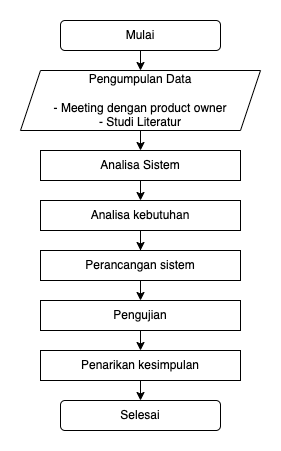
\includegraphics[width=0.4\textwidth]{gambar/tahapanpenelitian}
	\caption{Tahapan Peneltian}
	\label{fig:tahapan_penelitian}
\end{figure}


\section{Pengumpulan Data}

Data diambil dari hasil wawancara dengan owner J Farm Technology (JFT) Muhammad Eka Suryana, M.Kom., yang sekaligus merupakan klien dari penelitian ini. Selain itu, dilakukan studi literatur dengan membaca jurnal-jurnal yang terkait dengan topik penelitian. Setelah melakukan wawancara disimpulkan owner JFT membutuhkan suatu sistem web service untuk pengolahan data yang akan menerima request dari aplikasi mobile. Web service tersebut harus memiliki beberapa fitur diantaranya adalah pencatatan pemberian pakan setiap kolam, adanya fitur untuk meregistrasi kolam termasuk detail kolamnya, fitur untuk pencatatan masa budidaya pada setiap kolam termasuk dengan ikannya, fitur pencatatan kualitas air harian dan mingguan, pencatatan data kematian ikan, pencatatan treatment kolam, grading berat ikan kolam, perpindahan ikan antar kolam. Untuk transkrip wawancara dapat dibaca pada Lampiran 1.

\section{Analisa Sistem}

Sistem yang akan dihasilkan oleh penelitian ini berupa sebuah web service, lebih tepatnya adalah Private API. Sistem akan menggunakan arsitektur REST yang mana sering juga disebut RESTful. Sistem akan memberikan respons dari setiap request yang dilakukan oleh client. Request yang dilakukan oleh client memakai protokol http dan response yang diberikan oleh sistem berupa JSON Object. Yang nantinya sistem akan dijalankan di online server agar bisa di akses oleh client menggunakan akses internet.

\begin{figure}[H]
	\centering
	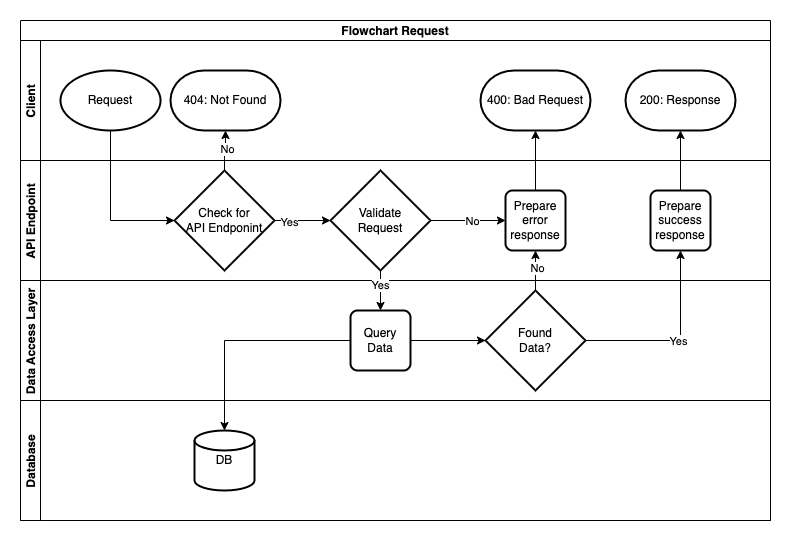
\includegraphics[width=0.85\textwidth]{gambar/flowchart_request_api.png}
	\caption{\emph{Flowchart} request}
	\label{fig:flowchart_request}
\end{figure}

Dimulai dari request yang dilakukan oleh client, ada beberapa proses yang akan dilakukan oleh sistem. Proses yang dilakukan oleh sistem diantaranya adalah pengecekan API EndPoint, validasi request, pengambilan dan penulisan data di database, dan persiapan response. Pengecekan API EndPoint dilakukan oleh sistem untuk mengetahui request apa yang diminta oleh client dari URL yang diakses. validasi request dilakukan untuk memastikan data yang dikirim oleh user telah sesuai dengan protokol yang telah ditentukan. Setelahnya proses yang dilakukan adalah memanipulasi atau membaca data di database. dan diakhiri dengan persiapan protokol response sebelum dikirim ke client.

\begin{figure}[H]
	\centering
	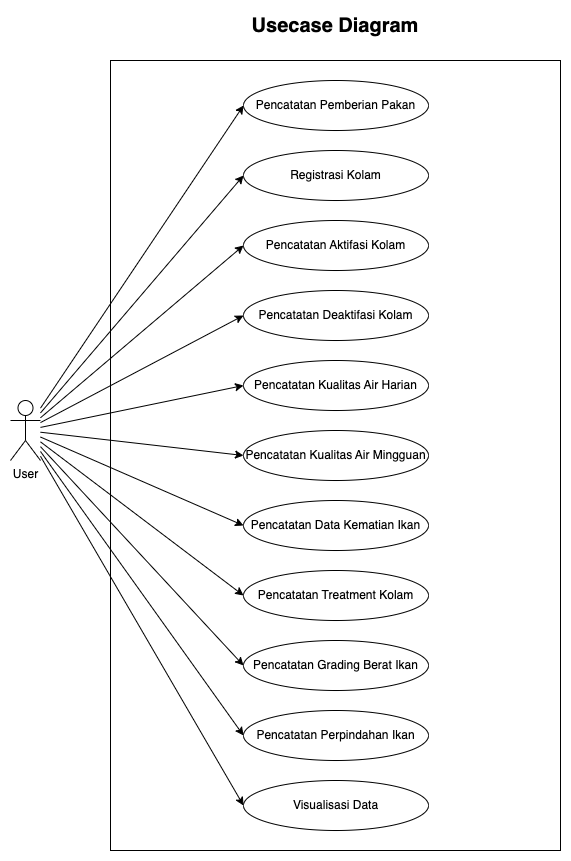
\includegraphics[height=0.9\textwidth]{gambar/usecase_diagram.png}
	\caption{\emph{Usecase} diagram}
	\label{fig:usecase_diagram}
\end{figure}

\textbf{Gambar \ref{fig:usecase_diagram}} merupakan usecase diagram user yang dibuat berdasarkan story yang telah didiskusikan bersama \textit{scrum master}. usecase tersebut menggambarkan kegiatan apa saja yang bisa dilakukan oleh user dalam menggunakan aplikasi. Pada penerapan pada \textit{backend usecase} nantinya akan di pecah lebih mendetail saat mendeskripsikan \textit{task} dari \textit{story}.

\section{Analisa Kebutuhan}

Berdasarkan uraian pada lampiran 1., prioritas fitur pada webservice perikanan modern terfokus pada pencatatan aktifitas pembudidaya ikan seperti pemberian pakan, pencatatan kematian ikan, dll.

Perangkat keras dan perangkat lunak yang penulis butuhkan adalah sebagai berikut:

\begin{enumerate}
\item Perangkat keras, terdiri dari:
\begin{enumerate} [a.]
\item Laptop dengan spesifikasi Processor Apple M1 \& Ram 8 GB
\end{enumerate}
\item Perangkat lunak, terdiri atas:
\begin{enumerate} [a.]
\item MacOs ventura 13.0
\item Visual Studio Code sebagai IDE dan code editor
\item Python sebagai bahasa pemrograman penyusun aplikasi web service
\item Flask sebagai framework python
\item MongoDB sebagai basis data
\end{enumerate}
\end{enumerate}

\section{Perancangan Sistem}

Untuk keberlangsungan penelitian, penulis menggunakan metodologi pengembangan sistem scrum Adapun tahapan-tahapan bagian dari scrum yang dilakukan dalam proses penelitian skripsi yang berjudul “Perancangan Arsitektur Backend Server Teknologi Perikanan Modren Berikut Spesifikasi Web Service yang Mampu Berhubungan dengan Multi Platform dengan Metode Scrum”. Flowchart metodologi Scrum yang dapat dilihat pada \textbf{Gambar \ref{fig:flowchart_scrum}}.

\begin{figure}[H]
	\centering
	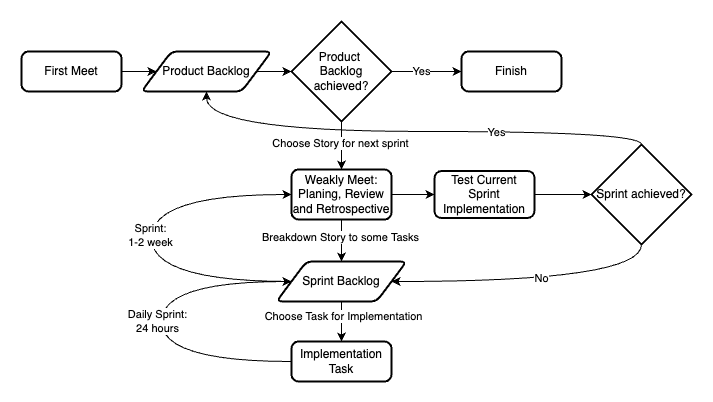
\includegraphics[height=0.6\textwidth]{gambar/design_penelitian_revisi.png}
	\caption{Flowchart Scrum}
	\label{fig:flowchart_scrum}
\end{figure}

Tahapan pertama penelitian adalah melakukan meeting dengan product owner dan scrum master. Meeting tersebut bertujuan untuk mendefinisikan product backlog yang akan menjadi acuan sprint kedepannya. Berikutnya merupakan weekly meeting pertama, agenda pada meeting ini adalah sprint planning. Sprint planning dilakukan dengan cara memilih story dari product backlog yang akan dilakukan breakdown sehingga menghasilkan sprint backlog. Sprint backlog merupakan kumpulan dari task-task kecil yang akan diimplementasi oleh developer setiap harinya. Weekly meeting berikutnya memiliki agenda tambahan dibanding dengan weekly meeting pertama yaitu, adanya sprint review dan sprint retrospective sebelum dilakukannya sprint planning untuk minggu berikutnya. Sprint review dan retrospective merupakan sebuah kajian dari task yang sudah dikerjakan oleh developer dan sprint yang dilakukan bersama oleh scrum master. Apabila tujuan dari sprint itu tercapai, maka scrum master akan menentukan story dari product backlog untuk sprint selanjutnya. Setelah semua product backlog tercapai maka sistem bisa dikatakan telah selesai.

Metode scrum terdiri dari beberapa komponen diantaranya adalah product backlog, sprint backlog, sprint, daily scrum, dan pengujian sistem. Berikut adalah penjelasan dari komponen-komponen tersebut:

	\subsection{Produk Backlog}
	
	Product backlog dibuat berdasarkan hasil diskusi dengan product owner sekaligus scrum master. Transkrip percakapan diskusi terdapat pada \textbf{Lampiran}. Setiap story yang ada di product backlog akan diselesaikan bertahap tiap minggunya. Berikut adalah tabel product backlog.
	
\begin{table}[H]
	\centering
	\caption{\textit{Product Backlog}}
	\label{table:product_backlog}
	\begin{tabular}{@{} |p{0.5cm}|p{10cm}|p{1cm}|p{2cm}| @{}}
		\hline
		\textbf{No} & \textbf{User Story} & \textbf{Sprint} & \textbf{Priority}\\
		\hline
		1 & Modul CRUD dan tampilan Pencatatan Pemberian pakan &  1,2 & High\\
		\hline
		2 & Modul CRUD dan tampilan untuk Registrasi kolam&  3 & High\\
		\hline
		3 & Modul CRUD dan tampilan untuk Masa Budidaya Kolam &  4 & High\\
		\hline
		4 & Modul CRUD dan tampilan untuk Pencatatan data kematian ikan &  5,6 & Medium\\
		\hline
		5 & Modul CRUD dan tampilan untuk Pencatatan Sortir ikan &  7 & Medium\\
		\hline
		6 & Modul CRUD dan tampilan untuk Pencatatan Grading berat ikan &  8 & Medium\\
		\hline
		7 & Modul CRUD dan tampilan untuk Pencatatan kualitas air harian &  9 & Low\\
		\hline
		8 & Modul CRUD dan tampilan untuk Pencatatan kualitas air mingguan &  9 & Low\\
		\hline
		9 & Modul CRUD dan tampilan untuk Pencatatan treatment kolam &  10 & Low\\
		\hline
	\end{tabular}
\end{table}
	
	Dari \textbf{Tabel \ref{table:product_backlog}} di atas, Produk Backlog terdiri dari empat komponen yaitu, User Story, Sprint, dan Priority. Story merupakan sebuah pekerjaan yang menggambarkan suatu fitur atau suatu module, yang mana nantinya akan diuraikan kedalam sprint dalam bentuk task. Komponen sprint merupakan perkiraan pada sprint keberapakah story akan dikerjakan. Priority merupakan sebuah keterangan seberapa prioritasnya user story.
	
	\subsection{Sprint Backlog}
	
	Sprint backlog merupakan sebuah task atau pekerjaan yang cenderung lebih kecil atau ringan. Sprint backlog merupakan uraian dari satu story pada product backlog yang menghasilkan beberapa task ringan. Sprint backlog diuraikan oleh scrum master. kemudian, developer bisa memilih task mana yang akan dikerjakan dahulu. Berikut merupakan tabel sprint backlog pertama.
	
	\begin{enumerate}
	
		\item Sprint-1
		
		Sprint-1 dilaksanakan selama delapan minggu yaitu pada tanggal 5 April sampai 31 Mei 2021. delapan minggu tersebut dikarenakan terdapatnya libur lebaran idul fitri selama 2 minggu yaitu pada tanggal 25 April - 9 May. Lalu enam minggu sisanya merupakan waktu yang dibutuhkan penulis untuk menulis penelitian, pembelajaran Scrum, pembelajaran framework flask, dan pembelajaran deployment pada server. Sprint ini merupakan uraian dari story "Pencatatan pemberian pakan" pada product backlog.
		
	\end{enumerate}
	
	\begin{table}[H]
	\caption{\textit{Sprint-1 backlog}}
	\label{sprint1_backlog}
	\begin{tabular}{@{} |p{0.5cm}|p{5cm}|p{5cm}|p{2cm}| @{}}
		\hline
		\textbf{No} & \textbf{\textit{Story}} & \textbf{\textit{Task}} & \textbf{\textit{Status}} \\
		\hline
		1 & \multirow{10}{5cm}{Create, Read, Updte, dan Delete untuk Pencatatan Pemberian pakan} & Merancang Database & Completed\\
		\cline{1-1}\cline{3-4}
		2 & & Merancang struktur flask framework & Completed\\
		\cline{1-1}\cline{3-4}
		3 & & Merancang class diagram & Completed\\
		\cline{1-1}\cline{3-4}
		4 & & Implementasi model Pond, Feed\_type, Feed\_history & Tested\\
		\cline{1-1}\cline{3-4}
		5 & & Implementasi controller EndpointApi & Tested\\
		\cline{1-1}\cline{3-4}
		6 & & Deployment Sistem & Tested\\
		\cline{1-1}\cline{3-4}
		7 & & Konfigurasi sistem di server & Tested\\
		\cline{1-1}\cline{3-4}
		8 & & Merancang Dokumentasi API & Tested\\
		\hline
	\end{tabular}
	\end{table}
	
	\subsection{Daily Scrum}
	
	Daily scrum tidak dilakukan secara meeting dikarenakan terbatasnya waktu scrum master dan developer. Maka dari itu, daily scrum digantikan dengan mencatat hambatan dan hal penting yang terjadi pada saat menjalankan sprint setiap harinya pada note github projects.
	
	\subsection{Sprint Review dan Sprint Retrospective}
	
	Sprint review dan retrospective dilakukan pada awal pekan tepatnya pada hari selasa. Sprint review dan retrospective dilakukan dengan cara voice call melalui platform telegram dan discord. Pembahasan dari meeting ini dimulai dari evaluasi perkembangan sistem, hambatan yang terjadi, dan penetapan sprint kedepannya.
		
\section{Pengujian}
Pada tahap ini peneliti akan melakukan uji backend server perikanan modern menggunakan dua jenis pengujian yaitu unit testing dan User Acceptance Test (UAT). Pengujian unit testing dilaksanakan oleh developer untuk memastikan fungsi-fungsi pada aplikasi yang telah dikembangkan dapat berjalan dengan baik. Sedangkan UAT dilaksanakan oleh scrum master untuk mengetahui apakah backend server sudah sesuai dengan kebutuhan dan layak untuk dipakai oleh developer frontend.

\begin{enumerate}
\item Unit Testing
Skenario pada unit testing dibuat berdasarkan skenario pemakaian web service yang ada pada fitur-fitur di product backlog. Skenario pemakaian web service adalah dengan melakukan request terhadap endpoint api yang ada pada setiap fitur. Setiap fitur setidaknya memiliki 4 skenario request yaitu GET, POST, PUT, DELETE. Adapun skenario dari unit testing yang akan diuji oleh developer terdapat pada \textbf{Tabel \ref{table:unit_testing}}.
\begin{longtable}{| p{3cm} | p{10cm} |}
\caption{Skenario unit testing.\label{table:unit_testing}}\\

\hline
\multicolumn{2}{| c |}{Awal Tabel}\\
\hline
\multicolumn{1}{|c|}{\textbf{Uji unit}} & \multicolumn{1}{|c|}{\textbf{Skenario Pengujian}}\\
\hline
\endfirsthead

\hline
\multicolumn{2}{|c|}{Lanjutan \textbf{Tabel \ref{table:unit_testing}}}\\
\hline
\multicolumn{1}{|c|}{\textbf{Uji unit}} & \multicolumn{1}{|c|}{\textbf{Skenario Pengujian}}\\
\hline
\endhead

\hline
\endfoot

\hline
\multicolumn{2}{|c|}{Akhir \textbf{Tabel \ref{table:unit_testing}}}\\
\hline\hline
\endlastfoot

Pemberian Pakan                  & Request POST API pencatatan pemberian pakan                                                    \\ \cline{2-2}
                                 & Request PUT API merubah data pemberian pakan                                              \\ \cline{2-2}
                                 & Request GET API mendapatkan list data pemberian pakan pada suatu kolam                                      \\ \cline{2-2}
                                 & Request GET API mendapatkan detail data pemberian pakan                                     \\ \cline{2-2}
                                 & Request DELETE API hapus data pemeberian pakan                                                  \\ \hline
Registrasi Kolam                 & Request POST API pencatatan registasi kolam                                                   \\ \cline{2-2}
                                 & Request PUT API merubah data kolam                                                           \\ \cline{2-2}
                                 & Request GET API mendapatkan list data kolam                                                  \\ \cline{2-2}
                                 & Request GET API mendapatkan detail data kolam                                                \\ \cline{2-2}
                                 & Request DELETE API hapus data kolam                                                             \\ \hline
Musim Budidaya Kolam            & Request POST API memulai musim budidaya pada kolam                                            \\ \cline{2-2}
                                 & Request POST API mengakhiri musim budidaya atau panen pada kolam                              \\ \cline{2-2}
                                 & Request GET API mendapatkan list musim budidaya pada suatu kolam                             \\ \hline
Pencatatan Kematian Ikan         & Request POST API pencatatan kematian ikan                                                     \\ \cline{2-2}
                                 & Request PUT API merubah data kematian ikan                                                   \\ \cline{2-2}
                                 & Request GET API mendapatkan list data kematian ikan pada suatu musim budidaya                \\ \cline{2-2}
                                 & Request GET API mendapatkan detail kematian ikan                                             \\ \cline{2-2}
                                 & Request DELETE API hapus kematian ikan                                                          \\ \hline
Perpindahan Ikan Antar Kolam     & Request POST API pencatatan perpindahan ikan antar kolam                                      \\ \cline{2-2}
                                 & Request PUT API merubah data perpindahan ikan antar kolam                                    \\ \cline{2-2}
                                 & Request GET API mendapatkan list data perpindahan ikan pada suatu musim budidaya             \\ \cline{2-2}
                                 & Request GET API mendapatkan detail perpindahan ikan                                          \\ \cline{2-2}
                                 & Request DELETE API hapus data perpindahan ikan                                                  \\ \hline
Grading berat ikan               & Request POST API pencatatan grading berat ikan                                                \\ \cline{2-2}
                                 & Request PUT API merubah data grading berat ikan                                              \\ \cline{2-2}
                                 & Request GET API mendapatkan list data grading berat ikan pada suatu musim budidaya           \\ \cline{2-2}
                                 & Request GET API mendapatkan detail grading berat ikan                                        \\ \cline{2-2}
                                 & Request DELETE API hapus data grading berat ikan                                                \\ \hline
Pencatatan kualitas air harian   & Request POST API pencatatan kualitas air harian kolam                                         \\ \cline{2-2}
                                 & Request PUT API merubah data kualitas air harian kolam                                       \\ \cline{2-2}
                                 & Request GET API mendapatkan list data kualitas air harian kolam pada suatu musim budidaya    \\ \cline{2-2}
                                 & Request GET API mendapatkan detail kualitas air harian                                 \\ \cline{2-2}
                                 & Request DELETE API hapus data kualitas air harian kolam                                         \\ \hline
Request POST Pencatatan kualitas air mingguan & API pencatatan kualitas air mingguan kolam                                       \\ \cline{2-2}
                                 & Request PUTAPI merubah data kualitas air mingguan kolam                                     \\ \cline{2-2}
                                 & Request GET API mendapatkan list data kualitas air mingguan kolam pada suatu musim budidaya  \\ \cline{2-2}
                                 & Request GET API mendapatkan detail kualitas air mingguan kolam                               \\ \cline{2-2}
                                 & Request DELETE API hapus data kualitas air mingguan kolam                                       \\ \hline
Pencatatan treatment kolam & Request POST API pencatatan treatment kolam                                       \\ \cline{2-2}
                                 & Request PUT API merubah data treatment kolam                                     \\ \cline{2-2}
                                 & Request GET API mendapatkan list data treatment kolam pada suatu musim budidaya  \\ \cline{2-2}
                                 & Request GET API mendapatkan detail treatment kolam                               \\ \cline{2-2}
                                 & Request DELETE API hapus data treatment kolam                                       \\ \hline
\end{longtable}
\item User Acceptance Test
Skenario pada User Acceptance Test dibuat berdasarkan fitur-fitur yang dapat diakses oleh owner. Fitur yang digunakan oleh owner adalah dashboard admin table yang menampilkan data-data yang telah di masukan ke dalam database. Adapun skenario dari UAT yang akan dilaksanakan terdapat pada tabel

\begin{longtable}{| p{8cm} | c | c | l |}
\caption{Daftar pengujian UAT.\label{table:skenario_uat}}\\
\hline
\multicolumn{4}{| c |}{Awal Tabel}\\
\hline
\multirow{2}{*}{Skenario Pengujian UAT} & \multicolumn{2}{l|}{Kesesuaian}            & \multirow{2}{*}{Kesimpulan} \\ \cline{2-3}
                                    & \multicolumn{1}{l|}{sesuai} & belum &                             \\ \hline
\hline
\endfirsthead
\hline
\multicolumn{4}{|c|}{Lanjutan \textbf{Tabel \ref{table:skenario_uat}}}\\
\hline
\multirow{2}{*}{Skenario Pengujian} & \multicolumn{2}{l|}{Kesesuaian}            & \multirow{2}{*}{Kesimpulan} \\ \cline{2-3}
                                    & \multicolumn{1}{l|}{sesuai} & belum &                             \\ \hline
\hline
\endhead
\hline
\endfoot
\hline
\multicolumn{4}{|c|}{Akhir \textbf{Tabel \ref{table:skenario_uat}}}\\
\hline\hline
\endlastfoot
Menampilkan dashboard tabel ketika mengakses http://jft.web.id/fishapi/ & & & \\ \hline
Tampilan tabel pencatatan pemberian pakan keseluruhan ketika mengeklik pencatatan pemberikan pakan pada sidebar dashboard &&&\\ \hline
Tampilan tabel pencatatan pemberian pakan harian ketika mengeklik pencatatan pemberikan pakan harian pada sidebar dashboard &&&\\ \hline
Tampilan tabel pencatatan pemberian pakan bulanan ketika mengeklik pencatatan pemberikan pakan bulanan pada sidebar dashboard &&&\\ \hline
Tampilan tabel kolam yang sudah di registrasi ketika mengkelik kolam -> detail pada sidebar dashboard&&&\\ \hline
Tampilan tabel masa budidaya kolam ketika mengkelik kolam -> masa budidaya pada sidebar dashboard &&&\\ \hline
Tampilan tabel jumlah Ikan setiap kolam ketika mengkelik kolam -> jumlah ikan pada sidebar dashboard &&&\\ \hline
Tampilan tabel data kematian ikan ketika mengkelik kematian ikan pada sidebar dashboard &&&\\ \hline
Tampilan tabel data sortir ikan ketika mengkelik sortir ikan pada sidebar dashboard &&&\\ \hline
Tampilan tabel data grading berat ikan ketika mengkelik grading ikan pada sidebar dashboard &&&\\ \hline
Tampilan tabel data kualitas air harian ketika mengkelik kualitas air -> harian pada sidebar dashboard &&&\\ \hline
Tampilan tabel data kualitas air mingguan ketika mengkelik kualitas air -> mingguan pada sidebar dashboard &&&\\ \hline
Tampilan tabel data treatment kolam ketika mengkelik treatment kolam pada sidebar dashboard &&&\\ \hline
\end{longtable}

\end{enumerate}
	

	
% Baris ini digunakan untuk membantu dalam melakukan sitasi
% Karena diapit dengan comment, maka baris ini akan diabaikan
% oleh compiler LaTeX.
\begin{comment}
\bibliography{daftar-pustaka}
\end{comment}

%-----------------------------------------------------------------
%Disini akhir masukan Bab
%-----------------------------------------------------------------


%-----------------------------------------------------------------
% Disini awal masukan untuk Daftar Pustaka
% - Daftar pustaka diambil dari file .bib yang ada pada folder ini
%   juga.
% - Untuk memudahkan dalam memanajemen dan menggenerate file .bib
%   gunakan reference manager seperti Mendeley, Zotero, EndNote,
%   dll.
%-----------------------------------------------------------------
\bibliography{daftar-pustaka}
\bibliographystyle{myapalike}
\addcontentsline{toc}{chapter}{DAFTAR PUSTAKA}
%-----------------------------------------------------------------
%Disini akhir masukan Daftar Pustaka
%-----------------------------------------------------------------


\end{document}